\documentclass[12pt]{book}
\usepackage{standalone}
\usepackage{apacite}
\usepackage{etoolbox}% for the \patchcmd
\makeatletter
% Patch after apacite got loaded!
\patchcmd{\nocite}{\@onlypreamble\document}{\documentclass\sa@documentclass}{}{}
\makeatother
\usepackage{graphicx}
\usepackage{subcaption}
\graphicspath{{/Users/huawei/Desktop/images/}} 
\usepackage{setspace}
\usepackage{booktabs}
\usepackage{tabularx}
\usepackage{xcolor}
\usepackage{amsmath}
\usepackage{pdflscape}
\usepackage[margin=3cm]{geometry}
\usepackage{multirow}
\usepackage{times}
\usepackage{fancyhdr}
\usepackage{color}
\usepackage{dcolumn}
\usepackage{siunitx}
\usepackage{array}
\usepackage{longtable}
\usepackage{tikz}
\usepackage{multicol}
\usepackage{tikzsymbols}
\usepackage{bm}
\usepackage{subcaption}
\usepackage{listings}
\usepackage{array}
\usepackage{siunitx}

\lstset{language=R,
	basicstyle=\small\ttfamily,
	stringstyle=\color{black},
	%otherkeywords={0,1,2,3,4,5,6,7,8,9},
	morekeywords={TRUE,FALSE, glmer, lmer},
	deletekeywords={data,frame,length,as,character},
	keywordstyle=\color{black}\bfseries,
	commentstyle=\color{black},
}


\usetikzlibrary{shapes.geometric, arrows}
\tikzstyle{startstop} = [rectangle, minimum width=1.5cm, minimum height=1cm,text centered, draw=black]
\tikzstyle{process} = [rectangle, rounded corners, minimum width=0.5cm, minimum height=1cm, text width =2.5cm, text centered, draw=black]
\tikzstyle{arrow} = [thick,->,>=stealth]
\usepackage{titlesec}    
\titleformat{\chapter}[display]
{\normalfont%
	\Huge% %change this size to your needs for the first line
	\bfseries}{\chaptertitlename\ \thechapter}{20pt}{%
	\huge %change this size to your needs for the second line
}

\raggedbottom

\renewcommand\baselinestretch{1.5}

\newcolumntype{d}[1]{D{.}{.}{#1}}
\def\sym#1{\ifmmode^{#1}\else\(^{#1}\)\fi}

%\usepackage{apacite}
\begin{document}
\chapter[Psychological implicit assessment]{Common measures for implicit psychological assessment} \label{chap:intro}

In this introductory chapter, a brief definition of automatic and controlled processes is provided, along with a summary of the main theoretical frameworks concerning the distinction of these processes. 

The Implicit Association Test \cite<IAT;>{Greenwald1998} is then presented, along with an overview of its use from the year of its first introduction (1998) to current days. The main fields of application of the IAT are illustrated as well. 
The issues related to the comparative measure that is gathered from the IAT is addressed by presenting an implicit measure able to provide an absolute evaluation towards one target object, namely the Single Category Implicit Association Test \cite<SC-IAT;>{karpinski2006}. The chapter ends with the illustration of the fully-crossed structure that characterizes the IAT and SC-IAT data.


\section{Automatic and controlled processes}
Throughout the past decades, social sciences have seen a growing interest in the possibility of assessing people's attitudes, preferences, opinions, personality traits and other psychological constructs without directly asking them but by inferring them from respondents' performance to computerized categorization tasks (i.e., implicit measures). 
Usually, implicit measures are tasks in which respondents' are called to sort stimuli representing different categories. The stimuli are specifically selected to trigger the activation of implicit processes, which are defined as processes operating outside of people's awareness but that can still affect behaviors, decisions, and social judgments \cite{greenwald95, greenwald2020}. The use of response times for inferring mental processes activated by a stimulus has a long tradition in psychology \cite<see >{greenwald2020}.
The implicit investigation of psychological and social constructs has been now widely recognized and it earned the label of ``implicit social cognition'' \cite{greenwald95}.

%The peculiarity of implicit processes is that they can be activated by a triggering stimulus, but they can remain outside of people's awareness. Despite the lack of awareness, implicit processes 

According to dual process theories \cite<e.g.>{devine1989, fazio2003}, two distinct but mutually reliant processes are involved in people's social behaviors and attitudes. This implies that they are different manifestations deriving from the same single--representation. Automatic and controlled processes usually happen simultaneously and involve automatic and controlled components.
Differently from implicit processes, which do not require the availability of cognitive resources for being activated, controlled processes do require a cognitive effort, resulting from the interaction between the person's willingness to engage in that process and the availability of cognitive resources and time for engaging in the  process \cite{fazio2003}. 
Moreover, controlled processes allow one to compare new information with previous experience and to make inferences on the environment in which they occur, making them more sensitive to social judgment and social desirability \cite<e.g.,>{greenwald2009}.

Controlled processes are usually assessed by means of what are defined direct measures, such as self-report scales. Consistently with the definition of controlled processes reported so far, direct measures assess the construct under investigation by directly giving an instruction to report it, presuming a certain degree of awareness of the construct itself \cite{greenwald2020}. 
Conversely, automatic processes are assessed with measures that assume no introspective awareness of the construct itself, and, most importantly, they measure the construct of interest without directly asking to report it \cite{greenwald2020}. 

A common trend for concurrently assessing controlled and automatic processes underlying psychological constructs is to administer a direct measure for capturing the former ones and an indirect measure for capturing the latter ones \cite{brownstein2019}. 

The controlled components of psychological constructs assessed by direct measures have been found to be highly correlated with the automatic components of the same psychological constructs assessed by indirect measures  \cite<e.g.,>{nosek2007implicit}. 
However, this correlation is reduced when the psychological constructs under investigation involve socially sensitive topics, such as racial prejudice \cite{greenwald2009, nosek2007implicit}. 
Another evidence pointing towards a dissociation between controlled and implicit processes comes from the type of behaviors predicted by these processes. 
Controlled processes assessed by direct measures have been found to be good predictors of deliberate behaviors (i.e., behaviors on which people have a certain degree of control), such as brand choice or food preference. Conversely, non-deliberate behaviors (i.e., spontaneous behaviors on which people do not have a control), such as prosemic and social distance in the interaction with members of stigmatized groups \cite<e.g.,>{dovidio2002}, are better predicted by implicit processes assessed with indirect measures \cite<e.g.,>{meissner2019, perugini2005, wilson2000model}.
Different hypotheses have been formulated for explaining the worse predictive ability of implicit measure in respect to behavioral deliberate choices, such as food/brand choices. 
For instance, \citeA{greenwald2017} claim that the automatic associations assessed by indirect measures can trigger deliberate thoughts about the associations themselves but they are unlike to predict behaviors. Conversely, decisions and choices might be more ascribable to the deliberate thoughts triggered by the automatic associations.  
\citeA{meissner2019} ascribe the scarce predictive ability of implicit measures in respect to deliberate choices to the type of implicit processes that these measures are tapping. Indeed, by the way in which they are designed, indirect measures tap the \emph{liking} component of the target objects, that is, how much an object is positively or negatively evaluated. Behaviors and choices are rather guided by a \emph{wanting} component, that is, how much a target object is desired. 

The apparent dissociation between automatic and controlled processes is still not solved, despite different theoretical frameworks have been trying to provide a conceptualization of these processes that should be able to explain these peculiar patterns of associations with external criteria \cite{perugini2005}.

According to dual process theories, it should not be surprising to observe such different patterns between controlled and automatic processes,and their predictive ability might change according to each and every kind of behaviors. Despite the two manifestations of the same attitude should provide a distinctive and unique prediction of the behavior, there might be cases in which one overrides the other in predicting the behavioral outcome. 
Moreover, controlled and automatic processes can be affected differently by other variables which are not directly accounted for by either the direct or indirect assessment, such as social desirability (direct measures) or a moment of distraction (indirect measures). 
Besides the external variables that can differently affect the direct and indirect assessment, the low correlation between the two measures of the same psychological construct can be due to the discriminant validity between two different types of measures, one based on introspection and on explicit and controlled responses, the other one based on response times and automatic responses.

Alternative explanations posit the coexistence of both explicit and implicit attitudes towards the same attitude objects \cite<Dual Attitudes Model;>{wilson2000model}. 
The combination between the degree of awareness of an implicit attitude and the extent to which motivation and cognitive resources are needed for overcoming the implicit attitude in favor of the explicit one generates different types of dual attitudes, namely repression, independent systems, motivated overriding, and automatic overriding.
The first dual attitude, \emph{repression}, requires the capacity of the explicit attitude to override the implicit one, which is kept outside of awareness. 
The dual attitude \emph{Independent systems} requires the presence of two attitudes towards the same object, one within awareness (explicit), and the other one outside of awareness (implicit). However, in this case, both systems develop evaluations, and they influence different type of responses (i.e., explicit and implicit responses). 
In both dual attitudes \emph{repression} and \emph{independent systems}, the implicit attitude did not reach awareness. 
In \emph{motivated overriding}, people are completely aware of the existence of the implicit attitude, but they are motivated to override it because they view it as illegitimate or they are ashamed of it. 
Clearly, this process requires the availability of cognitive resources for the explicit attitude to override the implicit one.
The difference between the \emph{motivated overriding} and the \emph{automatic overriding} lies in the automaticity of the overriding process. In the former case, it is a motivated and aware process, while in the latter case, the overriding occurs outside of people's awareness.

Two main assumptions underlie all dual attitudes. Firstly, once an implicit attitude is formed from previous experience, it does not require for cognitive resources to be activated, and it is activated every time the attitude object is encountered. 
Second, the explicit attitudes do require cognitive capacity and motivation to be retrieved. 
Both assumptions are in line with the conceptualizations of implicit and explicit processes presented so far.
The independence assumed between implicit and explicit attitudes towards the same attitudes object allows for speculating a double dissociation pattern in the prediction of behaviors. 
It follows that implicit attitudes can solely predict behaviors that are not under people's awareness and control, while explicit attitudes are directly related to behavioral responses under people's awareness and control. 
 


\section{The Implicit Association Test}\label{sec:iat}

%The assumption underlying the IAT functioning is rather simple: People tend to be faster in associating concepts that are related between each than in associating concepts that are poorly related, and the IAT has been specifically designed to capture and measure this tendency. Specifically, by observing the response latencies in a computed administered categorization task, the IAT assesses the strength of associations between concepts. 
Several implicit measures have been introduced for tapping the implicit component of attitudes, preferences, self-esteem, and other psychological constructs, such as the IAT \cite{Greenwald1998}, the Go/No-go Association Task \cite<GNAT;>{gnat}, and the Sorting Paired Features task \cite<SPF;>{spf}, just to name a few. 
Nonetheless, the IAT is the implicit measure that presents the best psychometric properties when compared to other commonly employed implicit measures \cite{bar2014}. 
Moreover, by appropriately changing the labels of the attitude objects and leaving its structure unaltered, the IAT is easily adaptable for the investigation of a broad range of topics \cite{zog}, such as stereotypes, attitudes, and self-concept. This characteristic of the IAT fostered its use in many different fields of applications, including law, criminal justice, education, marketing, and business  \cite<e.g.>{Epifania2020, greenwald2009, greenwald2020}.
%The IAT is specifically designed to tap the automatic aspects of attitudes, making it more resistant to self-presentation biases \cite<e.g.,>{greenwald2009}. As such, its use is particularly appealing for the investigation of socially sensitive topics, such as racial prejudice.

The IAT measures the strength of the associations between concepts by considering the speed and accuracy with which prototypical exemplars of two objects  categories (e.g., \emph{Coke} and \emph{Pepsi} images in a Coke-Pepsi IAT) and of two evaluative dimensions (i.e., \emph{Good} and \emph{Bad} attributes) are sorted in the category to which they belong by means of two response keys. 

The usual structure of an IAT (illustrated in Table \ref{tab:iatstructure}) is composed of 7 blocks.


%The usual structure of a Coke-Pepsi IAT is illustrated in Table \ref{tab:iatstructure}. 
\begin{table}[h!]
	\centering \doublespacing
	\caption{Coke-Pepsi IAT structure \protect\cite<adapted from >{Greenwald2003}.}
	\label{tab:iatstructure}
	\begin{tabular}{p{1cm}  p{4cm} p{4cm} p{4cm}}
		\toprule
		Block  & Function  & Left Response key & Right Response key \\
		\midrule
		B1  & Pure practice & Good words & Bad words \\
		B2  & Pure practice & Coke & Pepsi \\
		B3  & Associative practice & Good \& Coke & Bad \& Pepsi \\
		B4 & Associative test & Good \& Coke & Bad \& Pepsi \\
		B5 & Pure practice & Pepsi & Coke \\
		B6 & Associative practice & Good \& Pepsi & Bad \& Coke \\
		B7 & Associative test & Good \& Pepsi & Bad \& Coke \\
		\bottomrule
		\multicolumn{4}{p{14cm}}{\onehalfspacing\emph{Note:} The order of presentation of Blocks B3 and B4 and blocks B6 and B7 are counterbalanced across respondents.}
	\end{tabular}
\end{table}

The labels of the four categories, both the evaluative ones and the target objects ones, are fixed at the top left and right corners of the computer screen. 
	The stimuli are presented sequentially at the center of the screen. 
	
 The first two blocks are pure practice blocks in which respondents have to sort the stimuli belonging to either the evaluative dimensions (Block B1) or the stimuli belonging to the object categories (Block B2). These blocks have the purpose of letting the respondents familiarize with the stimuli and the task. Blocks B3 and B4 form the first associative condition. In these blocks, the object category \emph{Coke} shares the response key with \emph{Good} attributes, while the object category \emph{Pepsi} shares the response key with \emph{Bad} attributes (Coke/Good-Pepsi/Bad condition, CGPB). 
In Block B5, the labels of the object categories switch their positions on the computer screen. This block is a practice block  that lets respondents familiarize with the new locations of the labels. 
Blocks B6 and B7 constitute the contrasting associative condition, in which the categorization task is reversed. In these blocks, \emph{Pepsi} and \emph{Good} exemplars are sorted with the same response key, while \emph{Coke} and \emph{Bad} exemplars are sorted with the other response key (Pepsi/Good-Coke/Bad condition, PGCB). 
The assumption underlying the IAT functioning is that it is easier to sort together the exemplars of two categories when these categories are strongly associated with each other than when they are not. Consequently, respondents are supposed to perform better, in terms of faster time responses and higher accuracy, in the condition consistent with their automatically activated association(s).

The two associative conditions of the Coke-Pepsi IAT in Table \ref{tab:iatstructure} are depicted in Figure \ref{fig:IAT}. 

\begin{figure}[h!]
	\centering
	\begin{subfigure}[b]{0.4\linewidth}
		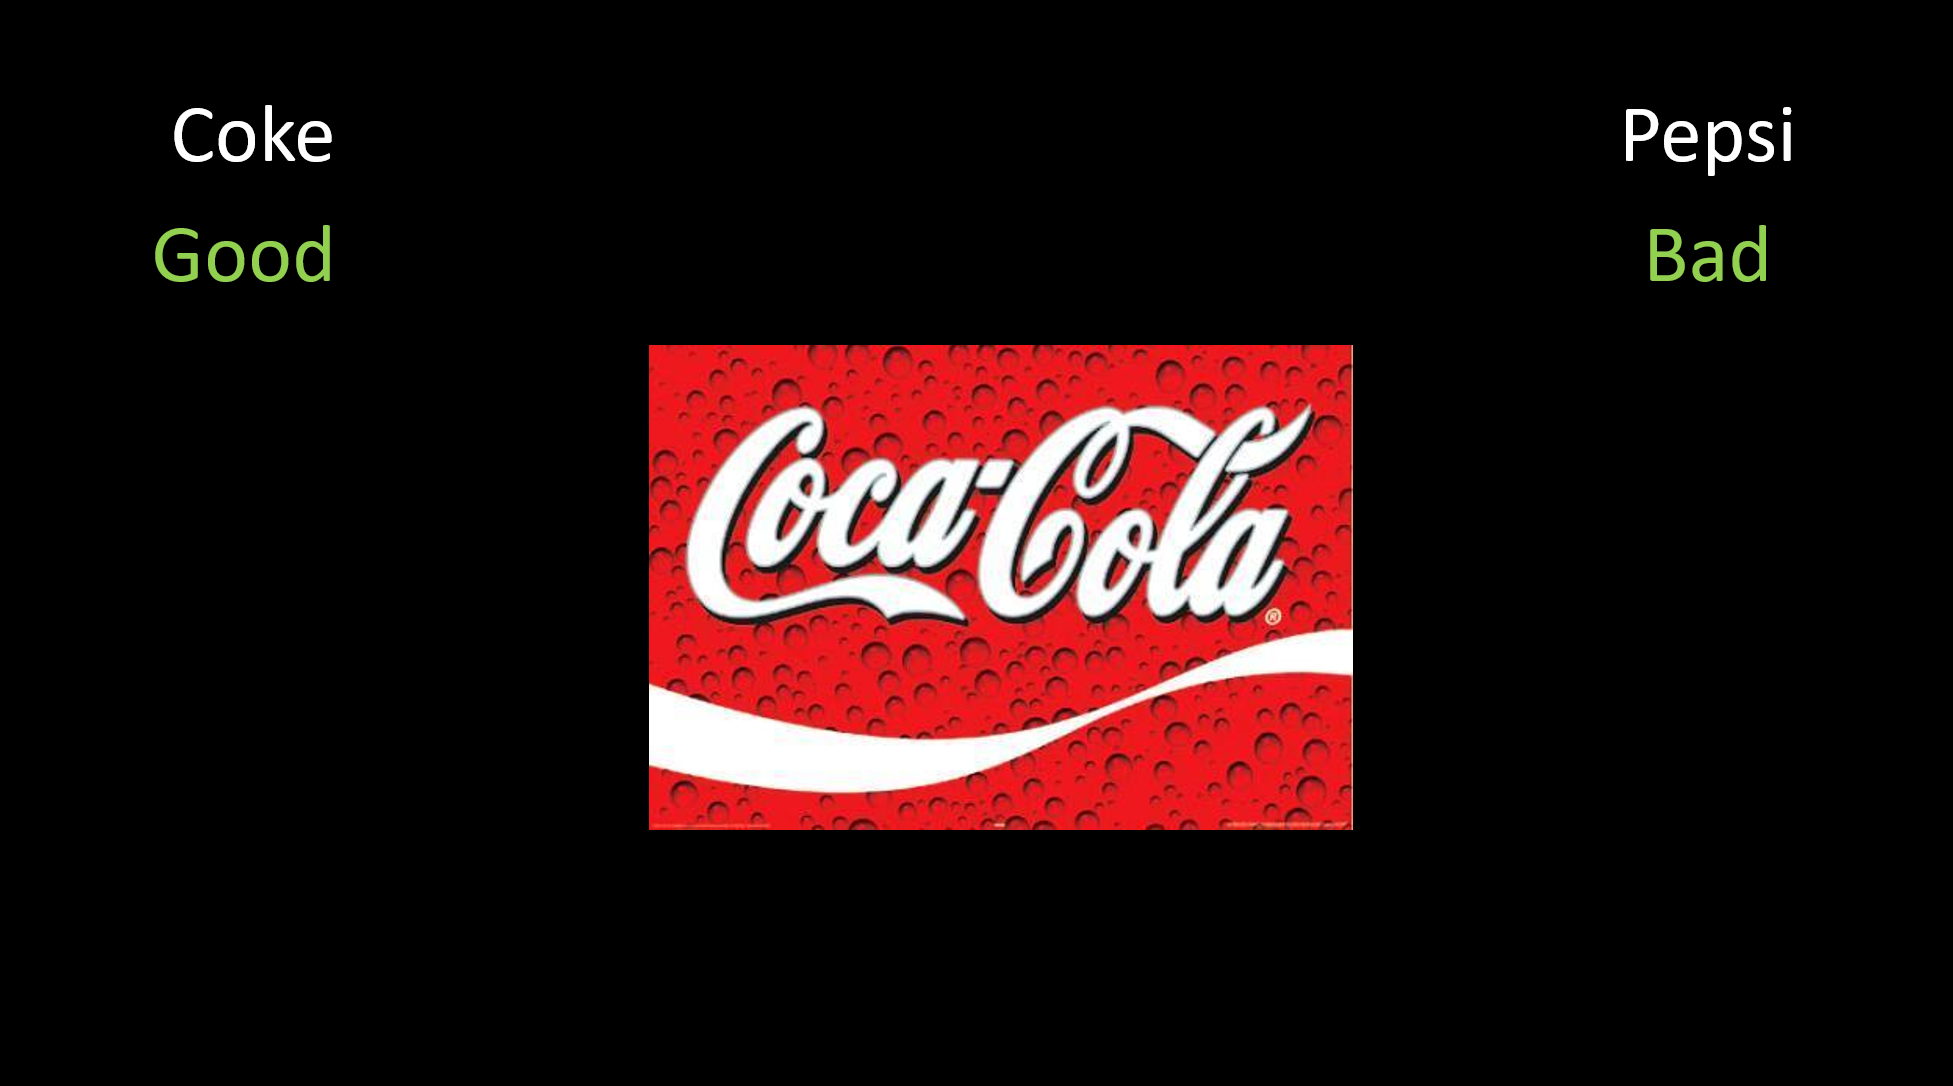
\includegraphics[width=\linewidth]{cocagood.png}
		\caption{Coke-Good/Pepsi-Bad condition}
		\label{cgpb}
	\end{subfigure}
	~ %add desired spacing between images, e. g. ~, \quad, \qquad, \hfill etc. 
	%(or a blank line to force the subfigure onto a new line)
	\begin{subfigure}[b]{0.4\linewidth}
		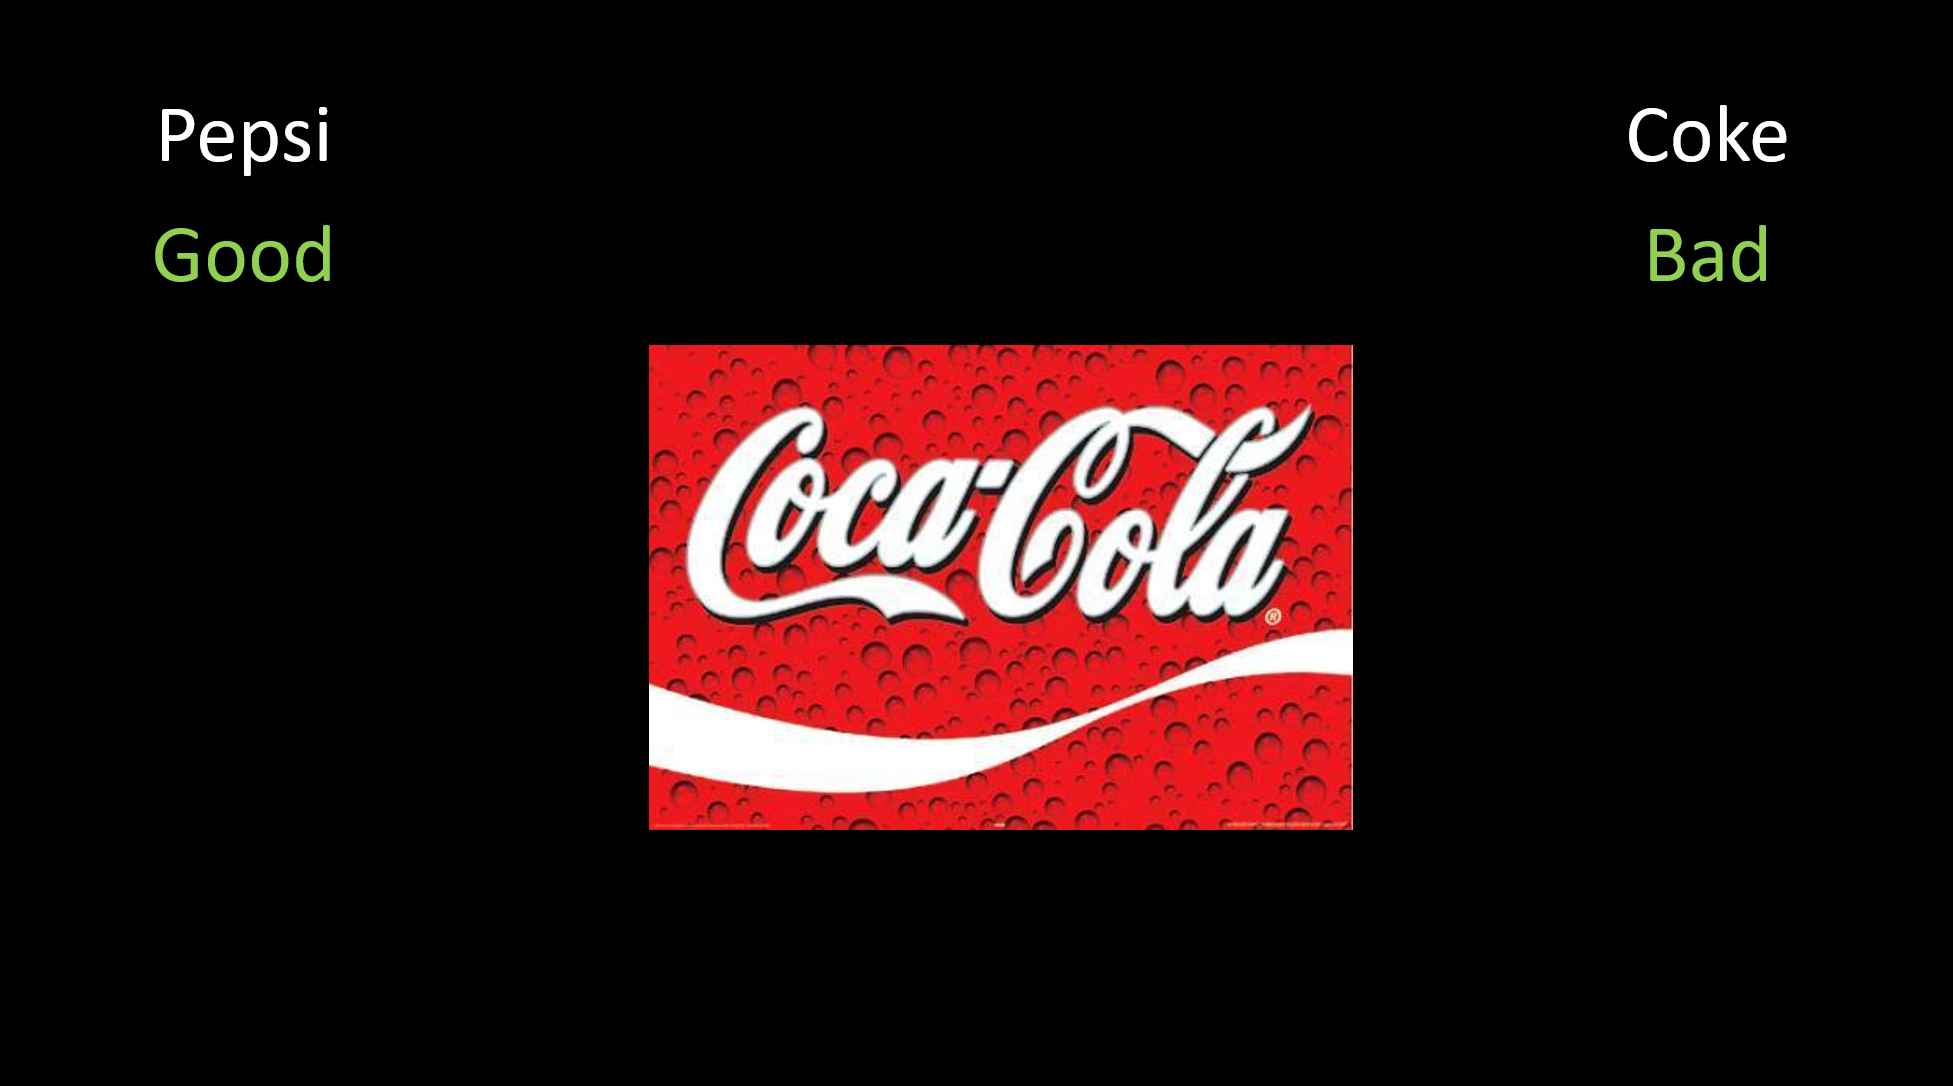
\includegraphics[width=\linewidth]{cocabad.png}
		\caption{Pepsi-Good/Coke-Bad condition}
	\end{subfigure}
\caption{\label{fig:IAT} Associative conditions of a Coke-Pepsi IAT.}
\end{figure}



During the administration of the IAT, respondents might be given feedback of their performance. If the IAT administration includes feedback, a red ``X'' appears every time a stimulus is sorted in the incorrect category. To proceed with the experiment, respondents have to correct their response. When the IAT does not include feedback in the administration, respondents are not notified when they commit errors, and they keep going with the experiment. 

The so-called IAT effect results from the difference in respondents' performance between the two conditions, and it is usually interpreted by means of the \emph{D} score \cite[see Chapter \ref{sec:iatD}]{Greenwald2003}.


\subsection{Fields of application}

A recent literature review \cite{Epifania2020} showed an increasing use of the IAT in wider and more varied fields of application.
Since the year of its first introduction (1998), the IAT has been used in more than 1,400 studies, investigating different topics. By reading the abstracts of 1,418 papers citing and using the IAT (i.e., number of citations from 1998 to October 25\textsuperscript{th} 2019, date of the search on Scopus database), it was possible to identify 6 main fields of application of the IAT: Social psychology ($n = 513$), Clinical and dynamic psychology ($n = 290$), Addiction ($n = 113$) , Food research ($n = 43$), Marketing research ($n = $34), and Other applications ($n = 425$). 
Figure \ref{fig:topicyear} depicts the trend lines for  each field of application from 1998 to 2019. 

\begin{figure}[!h]
	\centering
	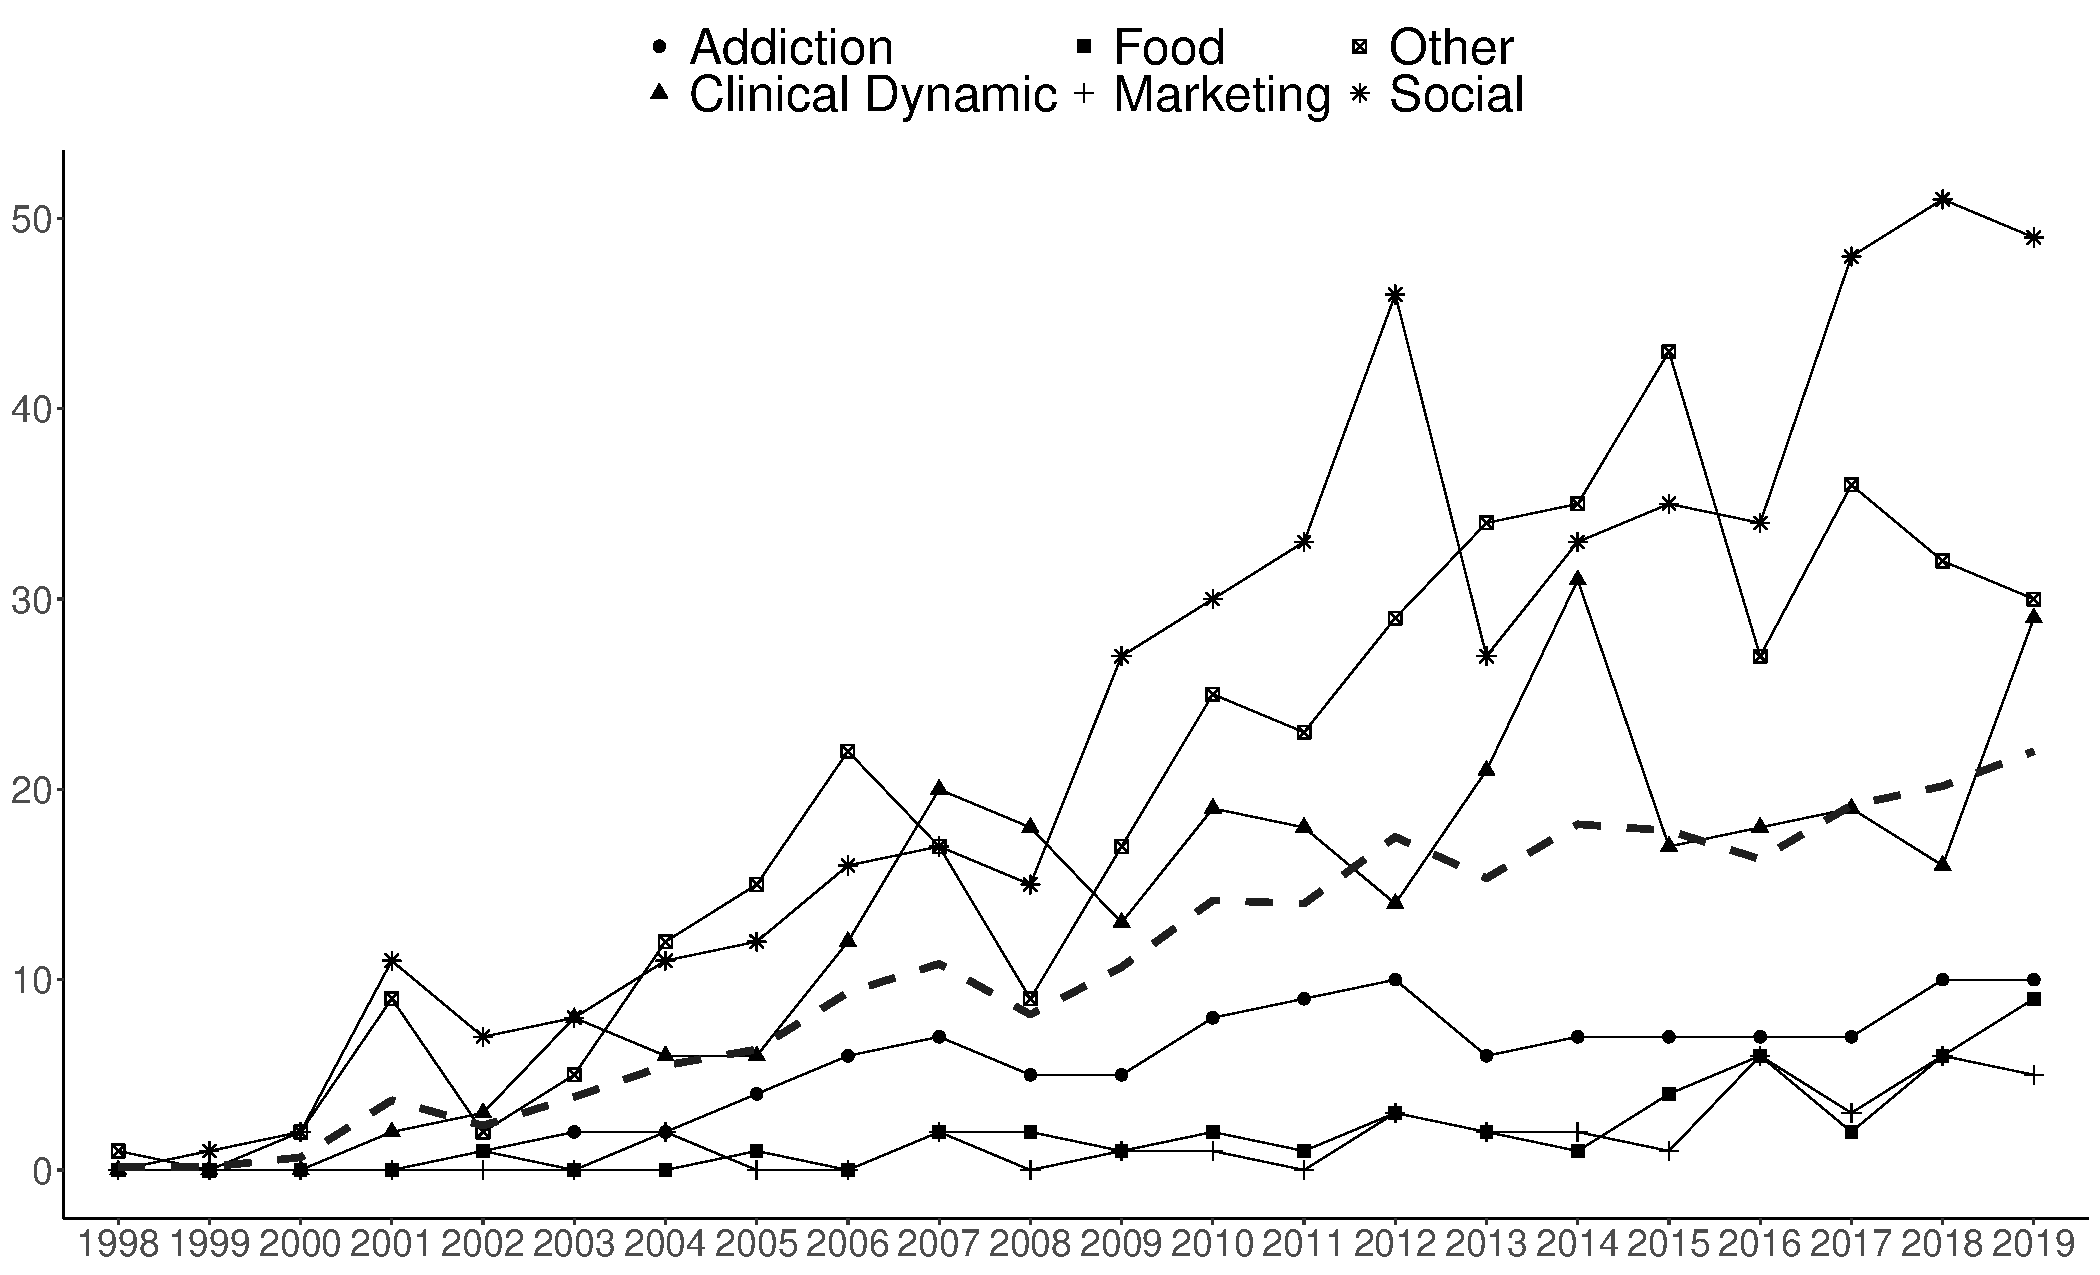
\includegraphics[width=\linewidth]{yearIATtopic.pdf}
	\caption{\label{fig:topicyear} Trend lines of each field of application of the IAT throughout from 1998 to 2019. }
\end{figure}

The dashed line in Figure \ref{fig:topicyear} represents the average trend of IAT use across the fields of applications. It clearly points at a constant and on-going growth in IAT use throughout the years. 

Trend lines of Social psychology and of Other appear always above the mean trend line. Clinical and dynamic psychology trend line is the most inconsistent one throughout the years. 
%Specifically, it shows a steady growth until 2007-2008, with a drop in 2009, followed by a vacillating trend until 2015, where it encounters a sort of \emph{plateau} with a final peak in 2019. 
The trend lines of Food and Marketing are similar between each other, both pointing at a higher use of the IAT during the past few years. 

Besides the general fields of applications of the IAT, it is interesting to delve deeper on the specific topics for which the IAT was employed (depicted in Figure \ref{fig:wordcloud}).

\begin{figure}[h!]
	\centering
	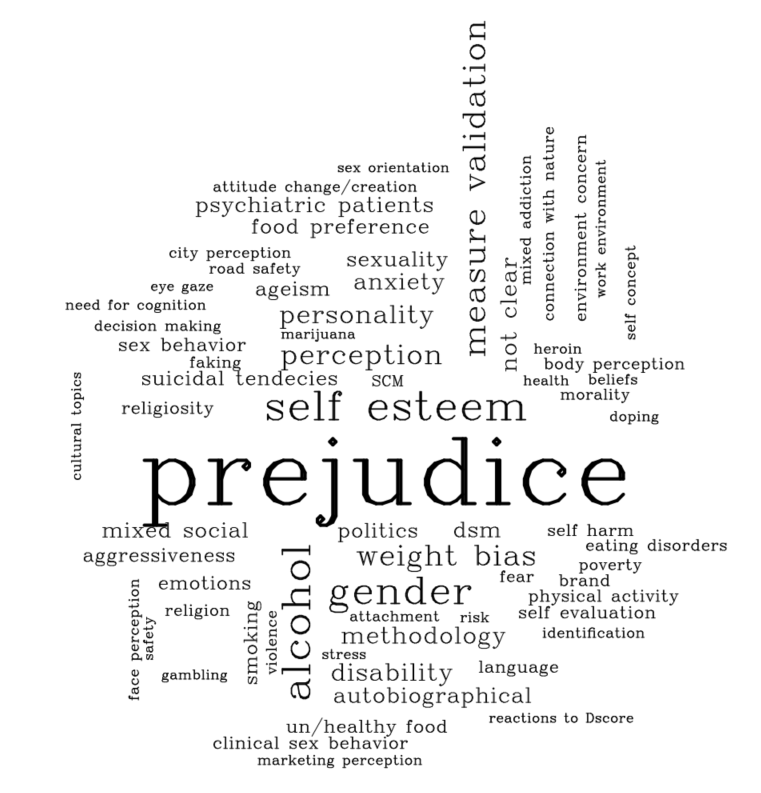
\includegraphics[width=0.5\linewidth]{wordcloudtopic.png}
	\caption{\label{fig:wordcloud} Word cloud of the fields of application of the IAT.  The bigger the word font, the more common the use of the IAT for the investigation of that specific topic.}
\end{figure}

Not surprisingly, the IAT was mostly used for investigating  implicit stereotypes and attitudes, such as implicit racial prejudice, gender stereotypes, attitudes towards obese people and other social groups (i.e., psychiatric patients and people with disabilities). 

The IAT has also been used for investigating addiction, unhealthy behaviors (i.e., smoking, alcohol consumption), personality traits, and self-perception.

The following paragraphs outline a brief summary of IAT use in each field of application. The complete report of the fields of application of the IAT, along with the samples used in the studies, can be found in \citeA{Epifania2020}.

\paragraph{IAT in Social psychology.} The resistance of the IAT to self-presentation strategies \cite<e.g.,>{greenwald2009} made it particularly appealing for investigating socially sensitive topics, such as racial prejudice and, more generally, stereotypes and attitudes towards different out-groups. 
Studies on this topic are followed by studies focused on gender stereotypes, and on the investigation of illness-related attitudes. 
In this thesis, illness-related attitudes is a label used for indicating attitudes towards people with either mental or physical disabilities, psychiatric patients, people with HIV, cancer patients and day-care patients in general, and suicide survivals.

Despite with lower frequency, the IAT is also used to assess attitudes towards people professing different religions, towards non-native English speakers, and bias towards people with low incomes. 
Papers composed by multiple studies in which attitudes towards multiple out-groups (e.g., out-group prejudice and weight bias) were concurrently investigated were common. The IAT was also used to investigate topics related to the Stereotype Content Model  \cite<SCM;>{fiske2002}, including infra-humanization, and to investigate the effectiveness of experimental manipulation to change/induce attitudes, even towards non-real groups.

%It is interesting to note the specific samples on which studies using the IAT have been carried out. Specifically, the IAT appears to be widely used among samples composed of hospital personnel (i.e., doctors, nurses, therapists), adults, undergraduates, and work personnel (i.e., CEOs, hiring personnel, university boards). 

%The common goal of studies investigating out-group prejudice and stereotypes, illness related attitudes, and weight bias among hospital personnel was to understand whether the implicit bias towards the specific out-group influenced the quality of the provided care on the probability of suggesting a specific surgery. The IAT was applied in a similar vein on samples composed of work personnel. Specifically, these studies were aimed at understanding whether implicit biases could undermine the probability of people belonging to minority groups, such as African-American people in the US, to be hired in a corporation or to win a position in Academia. Another interesting IAT application was for the investigation of the implicit out-group prejudice or implicit gender stereotypes of teachers. The aim of these studies was to understand whether teachers’ gender implicit attitudes (e.g., implicitly associating males with math and females with humanistic subjects) or their racial implicit attitudes (e.g., associating European-American children with higher intelligence than Hispanic children) could influence their behaviors towards their pupils.

\paragraph{IAT in Clinical and dynamic psychology.} The IAT was mostly used for the implicit assessment of self-esteem. Personality traits (e.g., Big Five personality traits), anxiety, and personality and mood disorders according to the Diagnostic and Statistical Manual of Mental Disorders (DSM) diagnosis definition were fairly investigated as well. 
The IAT was also commonly used for the implicit assessment of suicidal tendencies, aggressiveness, emotions, and clinical sex behavior (e.g., pedophilia). 

\paragraph{IAT in Addiction research.} The Vast majority of studies using the IAT in this field were focused on the investigation of alcohol addiction, followed by studies on nicotine and smoking addiction. The concurrent investigation of multiple addictions, such as drinking with smoking or drinking with gambling, was quite uncommon. 

\paragraph{IAT in Food research.} The IAT was mainly used to investigate the preference for different kinds of food, the preference for healthy over unhealthy food, or food perception in general. IAT was also employed for investigating attitudes towards dieting. Less common topics were food craving, food self--control, and the effect of the time of day on food preference. 

\paragraph{The IAT in marketing research.} Marketing research is one of the most recent fields of applications of the IAT. Most of the studies are focused on the implicit evaluation of the preference between different brands. Additionally, the IAT has been employed for studying the processes driving the decision to purchase some products, and the role of products labels and packaging in influencing the purchase of that specific product.

\paragraph{The IAT in macro-area Other.} The studies included in this field of application cover a broad and extensive range of topics, from gender perception of odds and even numbers \cite{gendernumber} to work related stress \cite{workstress} and romantic attachment \cite{romantic}.
Studies aimed at the validation of the IAT are included as well, and they compose the vast majority of studies in this field of applications. They are followed by studies on human perception and studies on methodology. The distinction between measure validation papers and methodology papers is quite subtle. Measure validation studies include papers aimed at the validation of the IAT procedure \cite<e.g.,>{Greenwald1998}, its score \cite<e.g.,>{Greenwald2003}, and the factors that may affect the IAT effect \cite<e.g.,>{bluemke2006}. 
Methodology papers includes studies in which existing formal models were used for modeling IAT data, such as the application of the Many-Facet Rasch Measurement Model \cite{linacre1989} in \citeA{anselmi2011} or the application of the Diffusion Model \cite{ratcliff1978} in \citeA{Klauer2007}. Studies aimed at the validation of \emph{ad-hoc} models for IAT data, such as the Quad Model \cite{Conrey2005} or the Discrimination-Association Model \cite{stefanutti2013} are included under the label methodology as well.

\section{The Single-Category Implicit Association Test}\label{sec:sciat}

The IAT has vastly proven its effectiveness and usefulness in providing a relative measure of the preference towards one object category compared with a contrasted one. 
%Many attitudes or preference objects present a clear contrasted category, so that it is meaningful and useful to investigate the relative preference/attitudes \cite{greenwald2000}. 
However, the measure obtained from the IAT presents two main shortcomings.
%However, the relative measure provided by the IAT is not able to understand whether the performance is driven by a positive evaluation towards one of the objects, a negative evaluation towards the opposite one, or a combination of the two evaluations.
%The resulting IAT effect is not able to actually acknowledge for the specific preference/dislike driving the responses.

Firstly, the relative measure provided by the IAT is not able to understand whether the performance is driven by a positive evaluation towards one of the objects, a negative evaluation towards the opposite one, or a combination of the two evaluations.
Sticking with the Coke-Pepsi IAT example in Section \ref{sec:iat}, faster responses in the Coke/Good-Pepsi/Bad associative condition might be due to either a preference for Coke (faster responses in sorting \emph{Coke} images and \emph{Good} attributes with the same response key), a dislike for Pepsi (Coke) (faster responses in sorting \emph{Pepsi} images and \emph{Bad} attributes with the same response key), or even a combination of the two.  One could try to decompose the IAT effect by computing separate scores for the trials in which \emph{Good} attributes and \emph{Coke} (\emph{Pepsi}) images are associated and in which \emph{Bad} attributes and \emph{Coke} (\emph{Pepsi}) images are associated. Even by doing so, it is not possible to obtain an absolute measure of the preference towards one of the two beverages \cite{nosek2005}. The IAT is based on a comparative task and, as such, it can only result in a comparative measure.
Consequently, the IAT is not the most appropriate choice when the focus in on the assessment of the absolute positive or negative evaluation of a single object. 
%When the focus of the research is on the assessment of the absolute positive or negative evaluation of a single object, the IAT might not represent the best choice. 
An appropriate example of a situation in which an absolute measure towards only one target object is preferable is self-esteem. 
In this case, the interest would be on how much a person values himself/herself. 
However, studies that employed the IAT for implicitly investigating this construct contrasted the category \emph{Self} or \emph{Me} with a generic category, like \emph{Other} \cite<e.g.,>{selfesteemOther} or \emph{Not Me} \cite<e.g.,>{selfesteemME}. 
Consequently, the measure resulted in an indirect evaluation of how much a person valued himself/herself in comparison to others, and not in how much a person valued himself/herself \cite{karpinski2006}. 

Secondly, since the IAT effect depends on the relative evaluation between the two categories, the choice of the contrasted category is of the uttermost importance. In some cases, a clear contrasted category is not available, and the researcher has to make arbitrary choices. 
Sticking with the Coke-Pepsi IAT example in Section \ref{sec:iat}, the relative attitude towards Coke strongly depends on the attitude towards Pepsi (and vice-versa). Take for example a respondent who does not like Pepsi at all and that does not hold either a negative or positive evaluation towards Coke. By using Pepsi as the contrasted category of Coke, a strong positive IAT effect can be found, although it would be mostly due to a dislike for Pepsi and not to a true positive attitudes towards Coke. By replacing Pepsi with another soft drink, the resulting IAT effect might change, and even result in a negative score.


Different alternatives have been introduced to overcome the issue of the relativeness of the IAT measure, like the SC-IAT \cite{karpinski2006}. 

The SC-IAT results from a slight modification of the IAT procedure. It is aimed at assessing  the strength of associations between concepts by considering the speed and accuracy with which different stimuli are sorted in their reference categories. 
The assumption that underlies the functioning of the SC-IAT is the same as that underlying the functioning of the IAT, namely, that it is easier to sort together exemplars of two categories when they are strongly associated with each other than when they are not. However, differently from the IAT, the exemplars of only one object category (e.g., \emph{Coke} in a Coke SC-IAT), along with the exemplars of two evaluative dimensions, are presented. 
The usual structure of a SC-IAT is illustrated in Table \ref{tab:sciatstructure}. 

\begin{table}[h!]
	\centering \doublespacing
	\caption{Coke SC-IAT structure \protect\cite<adapted from >{karpinski2006}.}
	\label{tab:sciatstructure}
	\begin{tabular}{p{1cm} p{4cm} p{4cm} p{4cm}}
		\toprule
		Block  & Function  & Left Response key & Right Response key \\
		\midrule
		B1  & Associative practice & Good \& Coke & Bad \\
		B2  & Associative Test & Good \& Coke & Bad \\
		B3  & Associative practice & Good  & Bad \& Coke \\
		B4  & Associative Test & Good  & Bad \& Coke \\
		\bottomrule
		\multicolumn{4}{p{13cm}}{\onehalfspacing\emph{Note:} The order of presentation of Blocks B1 and B2 and Blocks B3 and B4 are counterbalanced across respondents.}
	\end{tabular}
\end{table}

The SC-IAT is usually composed of 4 blocks. 
	In the first two Blocks (B1 and B2), the target object \emph{Coke} and the \emph{Good} attributes share the same response key, while \emph{Bad} attributes are sorted with the opposite response key (Coke/Good-Bad condition, CG). 
	In the last two blocks (B3 and B4), target object \emph{Coke} is sorted with the same response key as \emph{Bad}, while \emph{Good} words are sorted with the opposite response key (Coke/Bad-Good condition, CB).  

Blocks B1 and B3 are associative practice blocks, while Blocks B2 and B4 are the actual critical blocks that constitute the two associative conditions. 
%In the first critical block (B2), that is, the first critical condition, the target object \emph{Coke} and \emph{Good} attributes share the same response key, while \emph{Bad} attributes are sorted with the opposite response key (Coke/Good-Bad condition, CG). 
%In the contrasting associative condition (B4), target object \emph{Coke} is sorted with the same response key as \emph{Bad}, while \emph{Good} words are sorted with the opposite response key (Coke/Bad-Good condition, CB).  

The two conditions of the Coke SC-IAT described in Table \ref{tab:sciatstructure} are depicted in Figure \ref{fig:SCIAT}. 

\begin{figure}[h!]
	\centering
	\begin{subfigure}[b]{0.4\linewidth}
		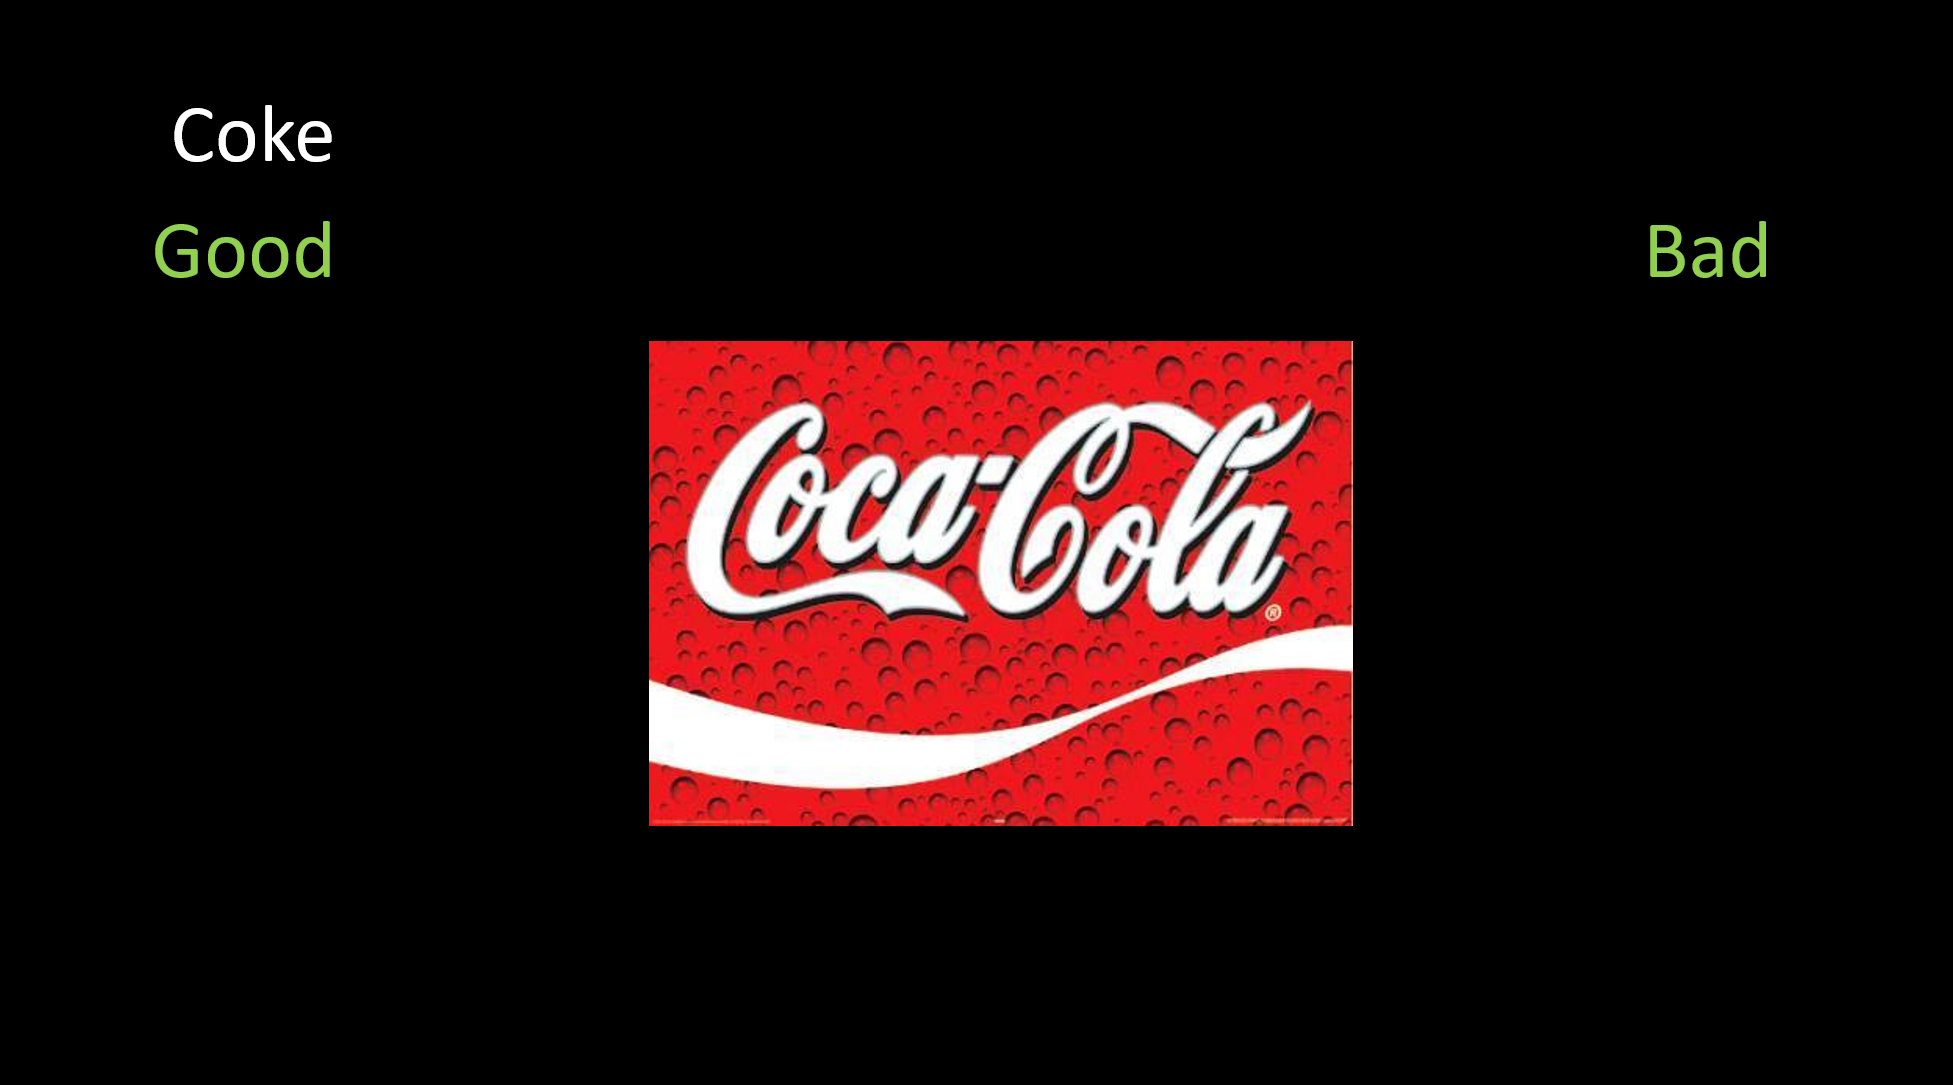
\includegraphics[width=\linewidth]{sccokegood.png}
		\caption{Coke-Good/Bad condition}
	\end{subfigure}
	~ %add desired spacing between images, e. g. ~, \quad, \qquad, \hfill etc. 
	%(or a blank line to force the subfigure onto a new line)
	\begin{subfigure}[b]{0.4\linewidth}
		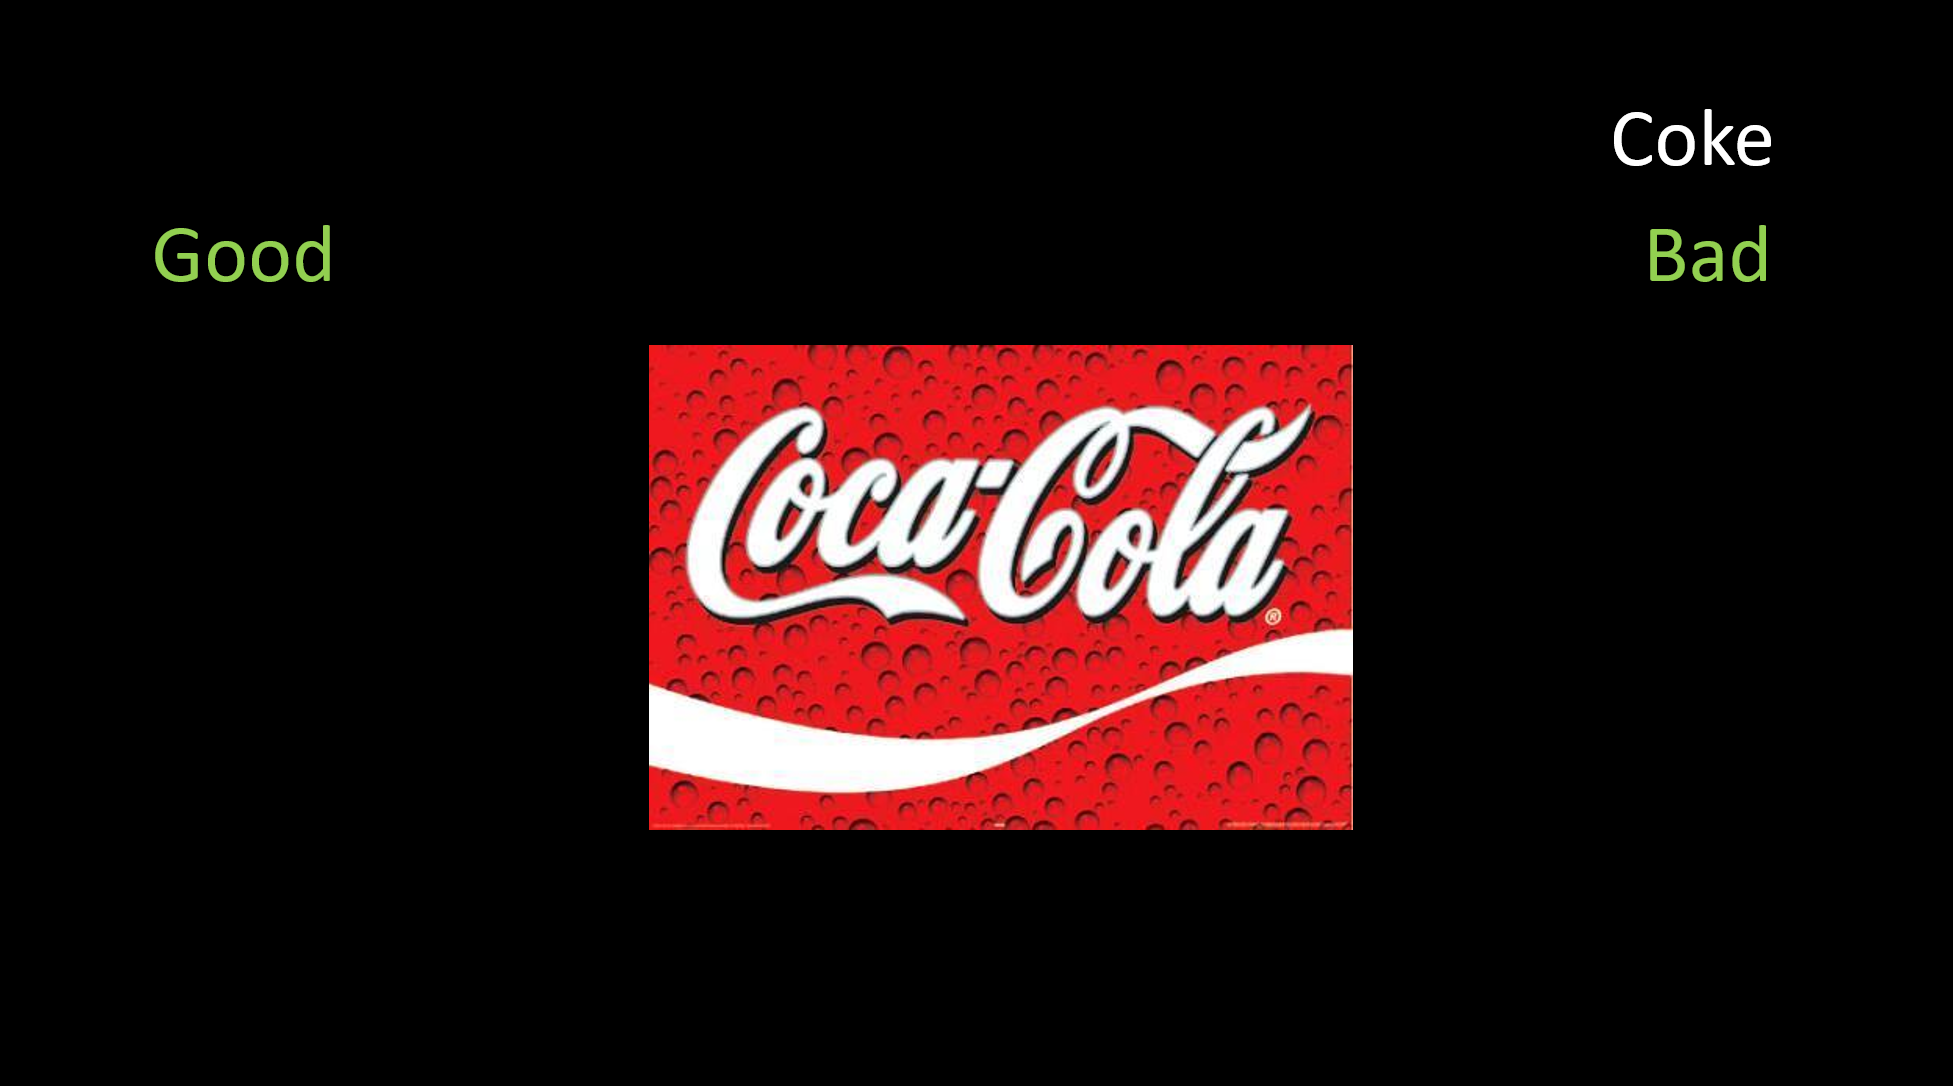
\includegraphics[width=\linewidth]{sccokebad.png}
		\caption{Coke-Bad/Good condition}
	\end{subfigure}
	\caption{\label{fig:SCIAT} Associative conditions of a Coke SC-IAT.}
\end{figure}

The SC-IAT administration usually includes a response time window (rtw) at 1,500 ms, after which the stimulus disappears and a warning message (e.g., ``Respond more quickly!'') is given to the respondent.
Every correct response is signaled by a green ``O'', while every incorrect response is signaled by a red ``X''. Differently from the IAT, respondents do not have to correct their incorrect responses to go on with the experiment. 

The rtw and feedback for every response are the two characteristics that differentiate the SC-IAT from the Single Target Implicit Association Test \cite<ST-IAT;>{stiat}. Nonetheless, the names (and procedures) of the two measures are used interchangeably \cite<e.g.,>{bar2014}.
The SC-IAT effect results from the difference in respondents' performance between the two contrasting conditions, and it is usually expressed by a modification of the IAT \emph{D} score \cite[see Chapter \ref{sec:sciatD}]{karpinski2006}.



\section[Fully-crossed design]{Implicit measures fully-crossed design}\label{sec:cross}


Suppose that two respondents, Lara and Francesco, are presented with the Coke-Pepsi IAT in Section \ref{sec:iat}. 

Lara might be, on average, more accurate (or faster) than Francesco. 
The difference in the overall performances of Lara and Francesco  can be ascribable to their individual differences and characteristics. 
The between--respondents variability is the expression of the differences due to individual characteristics, across the associative conditions. 

The set of exemplars chosen for representing each category presents their own variability as well. 
The \emph{Coke} logo can be immediately recognized and sorted in its own category, while an image of an old fashioned can of Coke might be less familiar and hence might need more time for being recognized and sorted. 
Similarly, the attribute \emph{evil} might be immediately recognized as belonging to the evaluative dimension\emph{Bad}, while attribute \emph{wicked} might not be immediately recognized as belonging to the evaluative dimension\emph{Bad} \footnote{The attribute \emph{evil} is the English translation for \emph{cattivo} (Italian). The attribute \emph{wicked} is the English translation for \emph{malvagio}. The spread Index (which varies from 0 to 1, where 1 indicates a high spread) for the former one is 0.85, while for the latter is 0.36 \cite{colfis}}. 
The between--stimuli variability is the expression of the sampling variability due to stimuli characteristics, across associative conditions. 

So far, only the between--respondents variability and the between--stimuli variability have been considered as the expression of individual differences and stimuli differences, respectively.
The effect of the IAT associative condition has not been mentioned yet. The change in respondent' performance according to the IAT associative condition is the main object of investigation when an IAT is administered. 

The respondents' individual differences might be exacerbated or diminished by the effect of the associative condition. 
Recall that Lara showed a better overall performance than Francesco. 
However, the difference in their performances might be attenuated in the Coke-Good/Pepsi-Bad condition. 
This attenuation might be due to several reasons. 
For instance, Lara might keep her performance unaltered because she is neither fond of Coke nor disgusted by Pepsi, while Francesco might show a better performance because he particularly likes Coke over Pepsi. 
In the opposite condition, the difference between the performances of Lara and Francesco might be exacerbated. Lara might still keep her performance unaltered, while Francesco might be struggle in associating his favorite soda with negative attributes. 
The within--respondents between--conditions variability is hence the expression of the variability in respondents performance that is ascribable to the effect of the associative condition. 

Usually, to investigate whether the associative condition had an effect on respondents' performance, a \emph{by-participant} approach is undertaken \cite<an individual respondents score is obtained by taking the difference in the average response time computed across trials in each condition;>{judd2012}.

There are no reasons to suppose that stimuli are immune to the effect of the associative condition. 
Some of the stimuli might be more easily sortable in one associative condition than the other for a number of reasons, including the specific attitude of the respondents. 
The within--stimuli between--conditions variability indicates whether the stimuli functioning changes according to the associative condition in which they are presented. 
By exploiting this information, it is possible to obtain a measure of the contribution given by each stimulus to the IAT effect. Following this line of reasoning, the more (less) a stimulus functioning changes between condition, the higher (lower) its contribution to the IAT effect. 

To investigate the effect of an experimental variable on the stimuli functioning, a \emph{by-stimulus} approach is undertaken \cite<an individual stimulus score is obtained by taking the difference in the average response time across respondents in each condition;>{judd2012}. 

There is still one source of variability missing, that is, the variability due to the respondents' reactions to each stimulus. 
Lara is a better respondent than Francesco, but she also does not have a particular preference for any of the sodas. It can  be speculated that Lara would generally react in the same way to each of the stimuli representing the two brand of sodas. 
On the other hand, Francesco has a strong preference for Coke. As such, he might be better than Lara in recognizing even the above-mentioned old-fashioned can of Coke. 
Consequently, he would have a better performance than Lara on this specific stimulus. 
The interaction between respondents and stimuli variability is hence the expression of the interaction between respondents and stimuli characteristics. 

This practical example was meant to give an overview of how the sources of variability in the IAT data are generated. A more detailed illustration of the IAT structure, and its related sources of random variability, is further illustrated. 
 
In the IAT\footnote{The SC-IAT presents the same data structure, although one of the target categories is dropped.}, the respondents are presented multiple times with the stimuli nested in two levels of two independent variables, namely the evaluative dimensions (\emph{Good} vs \emph{Bad}) and the target objects (e.g., \emph{Coke} vs \emph{Pepsi}). In a multilevel modeling perspective, respondents and stimuli can be considered at the same level.
%Since respondents are presented multiple times with the stimuli representing each of these categories, they are crossed with each level of the independent variables. Individual stimuli and individual respondents are at the same level and they are crossed with each other. 

Another independent variable, at a higher level, is the associative condition, which includes both the respondents and the stimuli, and it is in turn composed of two levels (e.g., CGPB condition and PGCB condition). 
Usually, the interest is on how the respondents' performance vary according to the associative conditions, which are the independent variables focus of attention when analyzing IAT data. 

%At a higher level that includes both stimuli and respondents, there is the associative condition, which includes other two levels (e.g., CGPB condition and PGCB condition). 

The stimuli representing each of the categories are presented multiple times both within and between the associative conditions. As such, besides being crossed with the respondents, the stimuli are crossed with the two levels of the associative condition. 
Similarly, the respondents are asked to respond to the stimuli multiple times both within and between the associative conditions. Therefore, besides being crossed with the stimuli, also the respondents are crossed with the associative conditions.  

Summarizing, the respondents and the stimuli are crossed with each other, and they are both crossed with the associative conditions. 
This data structure is usually referred to as a fully-crossed design, since all levels of the independent variables are crossed with each other \cite{Westfall2014}. 
The responses $x_{ps}$ of three participants $p$ to three stimuli $s$ (i.e., \Cat, \Snowman[1.5], \NiceReapey) in the two IAT associative conditions $c$ are represented in Table \ref{tab:fully} to exemplify the fully-crossed structure characterizing the measure.  

%An exemplification of the IAT fully-crossed structure is illustrated in Table \ref{tab:fully}. 

%In tasks like the IAT and the SC-IAT, stimuli representing each of the reference categories are presented multiple times, both within and between the associative conditions. Each stimulus is also presented multiple times to each respondent, both within and between the associative conditions. Thus stimuli and respondents are crossed with each other (multiple responses to the same stimulus by the same participant), and they are in turn crossed with the associative conditions (multiple responses on the same stimulus by the same respondent both within and between conditions). 
%Table \ref{tab:fully} reports a simple representation of a fully-crossed design, adapted from \citeA{Westfall2014}. 

\begin{table}[h!]
		\caption{Fully-crossed design.}
		\label{tab:fully} \centering \onehalfspacing
		\begin{tabular}{p{1cm}| p{1.5cm} p{1.5cm} p{1.5cm} p{0.05cm} p{1.5cm} p{1.5cm} p{1.5cm}}
			\toprule
		& \multicolumn{3}{c}{Condition A} & & \multicolumn{3}{c}{Condition B}\\
		\midrule
		\multirow{2}{*}{$p_1$} & \Cat[2] & \Snowman[2.5] & \NiceReapey[2] & & \Cat[2] & \Snowman[2.5] & \NiceReapey[2] \\
			 & \Cat[2] & \Snowman[2.5] & \NiceReapey[2] & & \Cat[2] & \Snowman[2.5] & \NiceReapey[2] \\
			 \hline
		\multirow{2}{*}{$p_2$} & \Cat[2] & \Snowman[2.5] & \NiceReapey[2] & & \Cat[2] & \Snowman[2.5] & \NiceReapey[2] \\
		 & \Cat[2] & \Snowman[2.5] & \NiceReapey[2] & & \Cat[2] & \Snowman[2.5] & \NiceReapey[2] \\
		 \hline
		\multirow{2}{*}{$p_3$} & \Cat[2] & \Snowman[2.5] & \NiceReapey[2] & & \Cat[2] & \Snowman[2.5] & \NiceReapey[2] \\
		& \Cat[2] & \Snowman[2.5] & \NiceReapey[2] & & \Cat[2] & \Snowman[2.5] & \NiceReapey[2] \\
		\bottomrule
		\multicolumn{8}{p{10cm}}{\emph{Note:} $p$: Respondents.}
	\end{tabular}
\end{table}


%\begin{table}[h!]
%	\caption{Fully-crossed design.}
%	\label{tab:fully} \centering \onehalfspacing
%	\begin{tabular}{l l l l l ll l l l l l  l}
%		\toprule
%	& \multicolumn{6}{c}{Condition A} &  \multicolumn{6}{c}{Condition B}\\
%	\hline
% Stimuli & \multicolumn{2}{c}{1} & \multicolumn{2}{c}{2} & \multicolumn{2}{c}{3} & \multicolumn{2}{c}{1} & \multicolumn{2}{c}{2} & \multicolumn{2}{c}{3}\\
% \hline
% Respondents & \multicolumn{12}{c}{}\\
% $p_1$ & $x_{11}$ & $x_{11}$ & $x_{12}$ & $x_{12}$ & $x_{13}$ & $x_{13}$ &  $x_{11}$ & $x_{11}$ & $x_{12}$ & $x_{12}$ & $x_{13}$ & $x_{13}$  \\
%  $p_2$ & $x_{21}$ & $x_{21}$ & $x_{22}$ & $x_{22}$ & $x_{23}$ & $x_{23}$ &  $x_{21}$ & $x_{21}$ & $x_{22}$ & $x_{22}$ & $x_{23}$ & $x_{23}$  \\
%   $p_2$ & $x_{31}$ & $x_{31}$ & $x_{32}$ & $x_{32}$ & $x_{33}$ & $x_{33}$ &   $x_{31}$ & $x_{31}$ & $x_{32}$ & $x_{32}$ & $x_{33}$ & $x_{33}$  \\
%		\bottomrule
%\end{tabular}
%\end{table}

Each cell of Table \ref{tab:fully} contains the unique combination respondent $\times$ stimulus for every repetition of the stimulus in each associative condition ($x_{psc}$). In other words, each cell contains the response to each IAT trial, that is the lowest level of observation, crossed with the stimuli, the respondents, and the associative conditions.
%the response $x_{psc}$, or, in other words, the response to each trial of the IAT. It constitutes the lowest level of observation. 
Each stimulus is presented multiple times in each condition to each respondent, hence multiple responses are observed for each of them. The illustration in Table \ref{tab:fully} clearly represents how the dependency at the level of the single observation is generated by the random noise in the data. 

%This design is rather common in experimental designs where samples of respondents respond to samples of stimuli in different condition \cite{Westfall2014}. 
Data deriving from a fully-crossed design, such as that of the IAT, should be carefully analyzed to account for the sources of variability, related to the participants, the stimuli, the associative conditions, and to their interaction \cite{Baayen2008, Barr2013, judd2017,  Westfall2014, wols2017}.  
These sources of variability generate dependencies between the observations that violate the assumption of conditional independence. 
This assumption is the basic assumption underlying data analysis in Social sciences, according to which, once the effect of the variability due to one latent variable is accounted for, the remaining variability can be explained by means of the experimental factors.

%As depicted in Table \ref{tab:fully}, the fully-crossed design characterizing the IAT (SC-IAT) results in a unique combination respondent $\times$ stimulus for every repetition of the stimuli in each associative condition, and different  sources of variability and dependency in the observed responses -- related to participants, stimuli, conditions, and to their interaction -- should be expected \cite{Barr2013, Westfall2014, wols2017}. 



%These are the main sources of variability that can be found in IAT or SC-IAT data and that have to be accounted for in order to obtain reliable estimates. 
%However, there is a part of variability that is due to the reactions of each respondent to each stimulus 
%Nonetheless, there's still a part of variability that is left out, which is the variability due to the presentation of each stimulus to each participant, or, in other words, the reaction of each respondent to each stimulus. 
Usually, the IAT (or SC-IAT) effect is expressed by means of an effect size measure that is obtained by aggregating the responses across the trials in each associative condition, and dividing these quantities by the standard deviation computed on the pooled trials of both blocks. This measure is the so-called \emph{D} score \cite<Chapter \ref{chap:classicscore};>{Greenwald2003, karpinski2006}, and it provides an easy-to-compute and easy-to-interpret measure of the implicit bias assessed by the implicit measure. 

However, the easiness with which \emph{D} score can be computed and interpreted comes with drawbacks that cannot be ignored. 
The computation procedure of the \emph{D} scores implicitly entails that the stimuli are taken as being the exhaustive representation of the population of stimuli (i.e., fixed factors), while respondents are considered as just one of the possible samples that could be drawn from a population (i.e., random factors) \cite{judd2012}. Considering the respondents as a random factor (hence treating them as random to make inferences on their reference population), and stimuli as a fixed factor, defines a \emph{by-participant} analysis. 

%Averaging across stimuli to obtain overall respondents' scores implies that stimuli are treated as fixed factors (i.e., the individual stimuli are taken to be the exhaustive representation of the population of stimuli), while respondents are treated as random factors (i.e., they are considered as just one of the possible samples that could be drawn from a population) \cite{judd2012, wols2017}.

Considering stimuli as fixed factors has important consequences both theoretically and statistically. 
 Firstly, treating stimuli as fixed factors assumes that they all have the same effect on the observed measure, or, in other words, they all have the same functioning. 
Moreover, the only inferences that are allowed concern the population from which the sample of respondents is drawn. The results are hence generalizable at the respondents' level but not at the stimuli level. 
Therefore, the replicability of the results to samples drawn from different populations is bounded to the use of the same exact set of stimuli \cite{judd2012}. 
Finally, averaging across trials leaves the variability due the between--stimuli variation uncontrolled.  

When the unaccounted error variance (the by-stimulus variation) is confounded with the effect of interest (the effect of IAT associative conditions), the risk of committing Type I error is inflated: The significant difference between the means can be due to the sources of error variance and not to the experimental effect \cite{Barr2013, judd2012,mc1989}. 

Not accounting for the sources of error variance also has important effect when the source is orthogonal (i.e., independent) to the effect of interest. In this case, the un-controlled error variance will reduce the power for testing the relevance of the effect of interest. Consequently, the importance of the experimental manipulation is underestimated \cite{Barr2013}. 

In the IAT (SC-IAT) case, the investigation at the stimuli level is not aimed at the functioning of each individual stimulus. Rather, the aim is to gather the information provided by each of the stimuli categories. The individual stimuli are assumed to be the realizations of the category to which they belong. 
As such, it makes sense to conceptualize the stimuli used in an IAT (SC-IAT) as possible samples drawn from the populations defined by the category to which they belong \cite{wols2017}. 
Given this conceptualization, considering stimuli as fixed factors, and not accounting for their sampling variation, appears to be a great fallacy when treating IAT (SC-IAT) data. Moreover, when the by-stimulus variation is not accounted for, all the information that can be gathered from them is overlooked \cite{wols2017}.
% the response given to a single, individual stimulus is not important \emph{per se}. Rather, the interest is on the categories that the stimuli are supposed to represent, with each individual stimulus being a realization of its category. The stimuli used in an implicit measure can be conceptualized as drawn from the population of stimuli representing their belonging category \cite{wols2017}. Moreover, by overlooking the sampling variation related to the stimuli, the information that can be gathered from them is completely neglected \cite{wols2017}.

The between--stimuli variability can be accounted for by performing \emph{by-stimulus} analyses \cite{judd2012}. 
Differently from the \emph{by-participant} approach (i.e., the respondents are treated as random factors and the stimuli are treated as fixed factors by averaging per participant across stimuli) presented so far, the \emph{by-stimulus} approach treats the stimuli as random factors and the participants as fixed factors. 
The stimuli are hence assumed to be just one of the possible sets of stimuli that can be drawn from a population of stimuli. 
The overall scores of each stimulus can be obtained by averaging per stimulus across participants. 
Clearly, the same pitfalls highlighted for the \emph{by-participant} approach apply for this instance, but reversed. 

Not considering the between--participants variability affects the computation of the mean score for each stimulus, and the statistical tests that can potentially be performed.  
However, the \emph{by-stimulus} analyses allow for the generalization of the results at the stimuli level, and  inferences can be made on the stimuli population. This makes the results replicable with other sets of stimuli drawn from the same population, but only if they are administered to the same sample of respondents \cite{judd2012}. 
 
As an attempt to overcome the replicability and generalizability issues concerning either the \emph{by-participant} approach or the \emph{by-stimulus} approach, \citeA{raaijmakers1999} suggested to report the results obtained with both the \emph{by-participant} and the \emph{by-stimulus} analyses. The results are then accepted as significant only if both analyses yielded significant results. 

The underlying logic appears to be quite straightforward. 
Given that the \emph{by-participant} analysis allows for generalizing to other populations of respondents (but only if the same stimuli are employed) and the \emph{by-stimuli} analyses allows for generalizing to others population of stimuli (but only if the same sample of respondents is used), then, if they are both significant, it is possible to generalize across both of them. 

Quite blatantly, this approach cannot do what it claims to do \cite{raaijmakers1999, raaijmakers2003}. 
The \emph{by-participant} analyses keep ignoring the sampling variation of the stimuli and the \emph{by-stimuli} analyses keep ignoring the sampling variation of the respondents. As such, their results are still flawed by un-wanted and uncontrolled error variance.
Besides, this approach presents also theoretical fallacies. 
%Significant \emph{by-participant} results do suggest would replicate only if the same set of stimuli is used. 
%Conversely, significant \emph{by-stimuli} results would replicate only if the same sample of respondents is used. 
The syllogistic reasoning according to which, if both the premises are true (both the \emph{by-participant} and the \emph{by-stimulus} analysis are simultaneously significant and the results can hence be replicated on different samples of respondents and stimuli, respectively), then also their conjunction would hold true (i.e., the results can be replicated with concurrently new samples of respondents and stimuli), appears too bold. 

A solution to this impasse is to consider both the respondents and the stimuli as random factors. 
By doing so, all the sources of variability at the different levels, and their potential interactions, can be accounted for, resulting in more reliable estimates \cite{Barr2013, judd2012, wols2017}.

Considering the respondents and the stimuli as random factors implies that both levels are assumed to be drawn from larger populations, on which the researcher is interested in making inferences \cite{judd2012, wols2017}. 
While the implications for the respondents are immediately clear, since they are typically considered as drawn from larger population, the same cannot be said for the stimuli. 
Indeed, the stimuli are usually considered as fixed factors. They are hence supposed to represent their population, and that they do all have the same effect on the outcome measures. 

Assuming that all employed stimuli in the IAT have the same effect on the outcome measure (i.e., the difference in the average response time in each associative condition) is an already proved fallacy \cite<e.g.,>{bluemke2006, ellithorpe2015}. 
When stimuli are considered as just one the possible samples that can be drawn from a larger population, it is implicitly entailed that they can vary for each observational unit. Therefore, they are allowed to have a different functioning, or, in other words, that they can make a difference in the observed measure, and that this difference and the information it conveys can be investigated \cite{judd2012}.  

The scores presented in Chapter \ref{chap:classicscore} are all affected by the above mentioned issues, as well as the formal models for the analysis of the IAT data presented in Chapter \ref{chap:formalModel}. 
	The approach used to address the fully-crossed structure of the IAT is presented in Chapter \ref{chap:ModelsIAT}.


\subsection{More than one implicit measure}
It is not uncommon to find studies in which the IAT and the SC-IAT are used concurrently to obtain both a comparative measure of the attitudes towards one object in comparison to its opposite, as well as an absolute measure of the positive/negative evaluations towards each of them  \cite<e.g.,>{bulmer2018implicit, fairer, glashouwer2013low}. 
To pursue this aim, one IAT and two SC-IATs, one for each of the target objects, are administered to the same respondents. The data of each implicit measure are separated and analyzed separately by computing individual scores for each measure. These scores are then employed for further analysis.

When both implicit measures are administered together, the fully-crossed structure represented in Table \ref{tab:fully} is repeated for each implicit measure. 
In other words, each implicit measure comes with its own sources of variability due to its fully-crossed structure.

Moreover, a super-ordinate variable, above the associative conditions, is added. The new super-ordinate variable is the type of measure. 
The associative conditions are hence nested within the specific implicit measure, while the respondents, besides being crossed with the stimuli and the measure-specific associative conditions, are also crossed with the implicit measures. Moreover, since the same stimuli are usually employed to represent the target objects and the evaluative dimensions in all implicit measures, also the stimuli are crossed with the implicit measures.
 

However, not all the stimuli are crossed with all implicit measures. While the stimuli belonging to the evaluative dimensions are indeed crossed with all implicit measures (i.e., they are administered in all implicit measures), the stimuli representing the target objects are presented only according to the specific measure. 
Specifically, stimuli representing both target objects are presented in the IAT, while only one of the target object categories is presented in each SC-IAT. The variable type of measure is hence introducing a nesting related to the stimuli. 
 
The implicit measure (e.g., the IAT rather than the SC-IAT) tends to be a variable of interest only in those studies aimed at either the validation of the measure itself or at the investigation of their different functioning.
Nevertheless, the by-measure variability that has been introduced needs to be taken into account to obtain reliable estimates and scores.

%When the IAT and the SC-IAT are administered together, each of them comes with its sources of dependence and variability due to the fully-crossed design characterizing each of them. 
%Moreover, if the IAT and the SC-IAT are administered with a \emph{within--subject} design, other sources of variability and dependency affect the data. 
%Firstly, the administration of each measure to the each respondent generates a variability within the responses of the same individual and between the implicit measures considered. This variability reflects the impact of each implicit measure on respondents' performance. 
%Moreover, since the same stimuli are usually employed for representing both the evaluative dimensions and the target object(s) in each measure, a within--stimuli between--measures variability should be expected as well. The within--stimuli between--measures variability should be considered as an indicator of a different functioning of the stimuli according to the specific implicit measure in which they have been presented. 

The scores computed on each implicit measure hence include the sources random variation due to both the fully-crossed design of each measure and the variability that should be expected by the multiple administration of the same set of stimuli to the same sample of respondents. 
The approach aimed at overcoming these issues with a comprehensive modeling of multiple implicit measures is presented in Chapter \ref{chap:comprehensiveModels}.

%\bibliographystyle{apacite} 
%\bibliography{biblioTesi}
\end{document}